\chapter{A románkori művészet} % Introduction
\label{ch:5_romankor}

\section{A románkori építészet, szobrászat és kézművesség}


\tcbox[left=0mm,right=0mm,top=0mm,bottom=0mm,boxsep=0mm,
toptitle=0.5mm,bottomtitle=0.5mm,title=\centering{A tétel adatai}]{%
	
	\begin{tabular}{| p{0.25\textwidth} | p{0.7\textwidth} |}

		\hline
		\centering{Tétel teljes címe}
		&
		Mutassa be a románkori építészet, szobrászat és kézművesség stílusjegyeit! Jellemezze a különböző műfajokhoz kapcsolódó alkotásokat, európai és hazai műemlékeinket!
		\\ \hline
		
		\centering{Jegyzetek}
		&
		\begin{compactitem}
			\item A románkor társadalma, hitvilága, építészete.
			\item A koraközépkori szobrászat, kódexfestészet és kézművesség jellemzői.
		\end{compactitem}
		\\\hline
		
	\end{tabular}}

	\subsection*{Bevezetés}
	
		\paragraph{Földrajzi elhelyezése}
		A román kor a népvándorlás kora után kialakuló nyugat-európai (elsősorban a német, francia nyelvterületek és itáliai), kereszténységet fölvett államok művészete.
		Az első keresztény állam létrejöttétől (Frank Birodalom Nagy Károly vezetésével kb. 800-tól) a IX., X., XI. századon át a XII. század végéig, a gótika elterjedéséig számítjuk.
		
		\paragraph{Korszakai}
		A IX., X. századot korai román, vagy preromán („pre” = valami előtti) kornak nevezzük.
		A XI., XII. század a korszak virágkora, ezért ezt érett román kornak nevezzük.
		
		\paragraph{Kifejezés eredete, jelentése}
		A kifejezés 19. századi eredetű. A nyugati nyelvekből került magyar nyelvbe, a nyugati szakkifejezés hangalakjának átvételével. A magyar kifejezésnek azonban semmi köze a román nyelvhez és népcsoporthoz, annál több az antik római kor építészetéhez. A román kori építészetben az ókori Róma építészetének hatását, vonásait fedezhetjük fel – a kifejezés jelentése tehát nem „román”, hanem római.
	
		\paragraph{Római hatások}
		\begin{compactitem}
			\item A román kor építészete az antik római építészet hatását mutatja: azzal kapcsolódik a római építészethez leginkább, hogy nyílásai, boltozatai félkörívesek. (A 19. században „félköríves stílnek” is nevezték megkülönböztetve az utána következő gótikától, ami a „csúcsíves stíl” nevet viselte).
			
			\item A román kor művészete abban „római”, „rómaias” még, hogy a vele egy időben virágkorát élő Bizánc művészetével szemben nem a keleti, ortodox, hanem a nyugati, Róma-központú keresztény egyház művészete.
			
			\item További „római” vonás a korban, hogy a korai román kor uralkodói – Nagy Károly, Ottók – arra törekedtek, hogy államaikkal az egykori antik nyugat-római birodalmat élesszék fel egyfajta „keresztény római birodalom” formájában.
		\end{compactitem}
	
	\subsection*{Kultúrtörténeti háttér}
		
		A román kor az Európába vándorolt „barbár” népek letelepülésével, államalapításával, a kereszténység felvételével kezdődik. A legjelentősebb ilyen megszilárdult keresztény állam a Frank Birodalom. A Frank Birodalom uralkodója Nagy károly, aki a római pápával 800-ban császárrá koronáztatja magát. Császársága az egykori nyugat-római birodalom jogutódja kíván lenni, és a Keleten virágzó Bizánc nyugati riválisa is, ezért fél évszázadnyi időre Nagy Károly Európa nagy részét fennhatósága alá vonja.
		
		\paragraph{A Német-Római Birodalom kialakulása}
		a X. században a német területek erősödnek meg: a német Ottó nevű uralkodók veszik át az irányítást. A frank állam hanyatlása, majd a kalandozó magyarok legyőzése után I. Ottó koronáztatja magát császárrá Rómában, és létrehozza a Német-Római Birodalmat szintén az egykori antik Róma felélesztésének szándékával. A Nyugat-Római Birodalom a XI-XII. században is Európa legnagyobb hatalommal bíró állama marad.
		
		\paragraph{A pápai állam vagy egyházi állam}
		A román kor alatt még egy jelentős állam jön létre: az Egyházi állam Közép-Itália területén. Ezzel a nyugati egyház politikai hatalomra is szert tesz Európában, és a művészetek legfőbb megrendelőjévé válik: templomokat épített, azok szobrászi és festészeti díszítését irányítja. Így a román kor művészete nagy részt szakrális, azaz vallásos célú. Tovább fokozza az egyház hatalmát Nyugat- és Közép-Európa területén az ún. egyházszakadás: 1054-ben az addig egységes keresztény egyház ketté válik: nyugati-római egyházzá és keleti, ortodox egyházzá.
		
		\paragraph{Szerzetesrendek}
		A román korban igen nagy szerepet töltenek be a népvándorlás alatt megszülető szerzetesrendek, melyek a betelepülő „barbár”népek megtérítésének, majd az új keresztény államokban a keresztény vallás terjesztésének érdekében jönnek létre. A terjesztésben a művészetet hívják segítségül: a templom-építészetben, kolostor-építészetben, a templomok, kolostorok szobrászati díszítésében, a kódexfestészetben jeleskednek. A leghíresebb román kori szerzetesrend a bencés rend (Szent Benedek alapítja).
		
		\paragraph{Keresztes hadjáratok}
		A román kor idején az egyház keresztes hadjáratokat indít, melyek a pápa által szentesített, a keresztes lovagok részvételével folytatott nagyarányú hadjáratok voltak a 11–13. században. Fő céljuk a Szentföld megszerzése volt a muszlim araboktól és törököktől, de a spanyol nyelvterületen előrenyomuló mórok (spanyolországi arabok, afrikaiak) ellen is.
		
		
	\subsection*{Templomépítészet}
	
	Ebben a koprszakban templomok, kolostorok és várak épülnek leginkább.
	
	\subsubsection{Külső jellemzők}
	
	A templom az egyház megerősödő hatalmát, az egyház által nyújtott védelmet van hívatva kifejezni, ezért külseje biztonságot, erőt, megingathatatlanságot sugall.
	\begin{compactitem}
		\item A külső zárt, csak kisméretű nyílásokkal van áttörve.
		\item A tömegek zárt, egyszerű, tömbszerű, gyakran egészen a geometriai.
		formákig leegyszerűsített hasáb-, henger- és kockaszerű egységek.
		\item A templomot vaskos, masszív, robosztus tömegek alkotják.
		\item A külső puritán, azaz alig díszített.
	\end{compactitem}

	\subsubsection{Alaprajz}
	
	A templom alaprajza a keresztény egyház szertartásainak rendje szerint alakul: követi az ókeresztény bazilikák formáját.
	\begin{compactitem}
		\item Hosszanti elrendezésű,
		\item három vagy öt hajós,
		\item keletelt: azaz keleti oldalán helyezkedik el a félkörívű apszis, a szentély,
		\item az apszis előtt négyezeti tér és kereszthajó található.
	\end{compactitem}

	\subsubsection{Szerkezet}
	
	\begin{wrapfigure}{r}{0.2\textwidth}
		\tcbox[colback=darkgray!85!black,
		left=0mm,right=0mm,top=0mm,bottom=0mm,boxsep=1mm,toptitle=0.5mm,bottomtitle=0.5mm,
		title=\centering{Kockafejezet}]{
			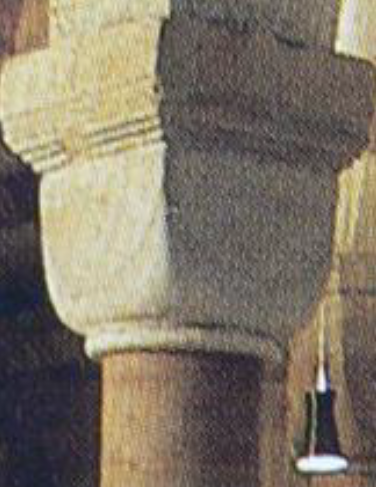
\includegraphics[width=1.0\linewidth]{05/kockafejezet}
		}
	\end{wrapfigure}
	
	A templomok bazilikális szerkezetűek, azaz
	főhajójuk kiemelkedik a mellékhajók fölött, és a belső
	tér a kiemelkedő falakon nyitott ablakokon keresztül
	kapja a megvilágítást.
	
	Az ablakok kis méretűek, a falak tehát kevéssé vannak áttörve, vastagok,
	masszívak, erősek, további külső megtámasztás nélkül viselik a boltozat súlyát.
	
	A román templomok belső súlyt hordó tartóelemei
	egyszerű, hasábszerű pillérek, vagy tömzsi oszlopok. Az oszlopfejezetek gyakran minden díszítést nélkülöző, kocka formájú oszlopfők – ezek az ún. „\textbf{kockafejezetek}”.
	
	\subsubsection{Külső díszítőelemek}
	
	A templomok kevéssé díszítettek, de a falfelületeket nyílások, függőleges és vízszintes elemek tagolják.
	
	\paragraph{Bélletes kapuzat}
	A román kori templomok legjellemzőbb homlokzati
	eleme, a befelé szűkülő, a kapu körül ívben végigfutó féloszlopokkal díszített
	félköríves kapuzat. A bélletek (a kapu fölött futó féloszlopok) gyakran
	geomertikus mintákkal, fogsor-motívummal, cikk-cakk mintával faragott.
	
	\paragraph{Lőrészszerű ablak}
	Kis ablaktípus, keskeny, felül íves, befelé szűkül.
	
	\paragraph{Ikerablak}
	Kettős vagy hármas ablak, felül ívesek (félkör) az ablakok
	között kis oszlopok vannak.
	
	\paragraph{Ívsor vagy ívpárkányzat}
	Vízszintes tagolóelem, ami a külsőn jelzi a belső
	szinteket: kis ívek sorakoznak egymás mellett.
	
	\paragraph{Törpegaléria}
	Apró árkádok (kis boltívek és kis oszlopok), árkád a homlokzaton, ami mögött egy keskeny fal húzódik.
	
	\paragraph{Vakárkád}
	A homlokzaton ált. alul található olyan árkádok ami alatt, nem lehet
	átmenni, mert be vannak falazva tehát csak díszítő szerepük van.
	
	\paragraph{Féloszlop}
	A falhoz tapadó, függőlegesen félbevágott oszlop (oszlop-lábazata,
	oszlopfője van).
	
	\paragraph{Pilaszter}
	A falból négyzetesen kiugró (oszlopszerű) falsáv, amelynek fejezete és
	lábazata van.
	
	\paragraph{Lizéna}
	A falból négyzetesen kiugró falsáv fejezet és lábazat nélkül.
	
	
	\subsubsection{Térlefedés}
	
	A templomok boltozási rendszere az antik Róma idején kialakult boltozást: a donga és keresztboltozatot fejleszti tovább.
	
	A leggyakoribb boltozattípus a „román
	keresztboltozat” = két félhenger alakú dongaboltozat
	kereszteződése négyzet alaprajzon.
	
	A román keresztboltozatnak két típusa alakult ki.
	
	\paragraph{Élkeresztboltozat}
	Az íves falrészek megerősítés nélkül élekben találkoznak.
	
	\paragraph{Bordás keresztboltozat}
	az íves falrészek találkozásánál a boltozatot bordákkal erősítik meg, a bordák, amiket erős, súlyosabb kövekből raknak ki levezetik a boltozat súlyát az oldalfalakra, így a köztük lévő falakat könnyebb kövekből lehet rakni (Ez a típus alakul ki időben később, a XII. sz.-ban).
	
	\paragraph{Kötött térrendszer}
	A boltozás rendszere, logikája: ún. „kötött térrendszer” v. ,,kötött boltozás”. Mivel csak négyzet alaprajzú tereket tudtak lefedni, kialakult az a rendszer, hogy a főhajó egy boltszakaszára a mellékhajóban két fele akkora négyzetes boltszakasz kerül: hevederívek, a boltszakaszokat egymástól elválasztó ívek.
	
	\begin{figure}[H]
		\centering
		\begin{minipage}{0.45\textwidth}
			\tcbox[colback=darkgray!85!black,
			left=0mm,right=0mm,top=0mm,bottom=0mm,boxsep=1mm,toptitle=0.5mm,bottomtitle=0.5mm,
			title=\centering{Keresztboltozat}]{
				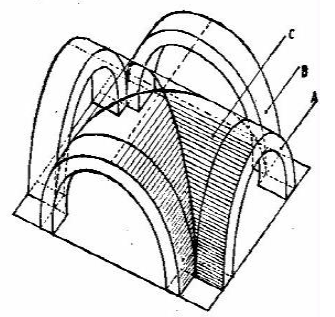
\includegraphics[width=1.0\linewidth]{05/keresztboltozat}
			}
		\end{minipage}
		\hfill
		\begin{minipage}{0.5\textwidth}
			
			\tcbox[colback=darkgray!85!black,
			left=0mm,right=0mm,top=0mm,bottom=0mm,boxsep=1mm,toptitle=0.5mm,bottomtitle=0.5mm,
			title=\centering{Kötött térrendszer}]{
				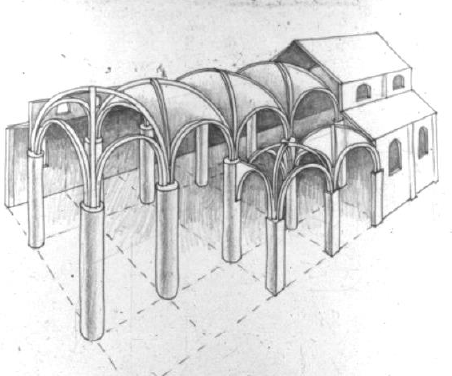
\includegraphics[width=1.0\linewidth]{05/kotott_terrendszer}
			}
		\end{minipage}
	\end{figure}

	\subsubsection{Német építészet}
	
	A német román templomok leghíresebb példái:
	a Német- Római császárok által épített dómok, ún. ,, császárdómok”: Hildesheim-i Szent Mihály templom, Maria Laach dómja, Speyer-i császárdóm, Worms-i császári dóm.
	
	\begin{figure}[H]
		\centering
		\begin{minipage}{0.3\textwidth}
			\tcbox[colback=darkgray!85!black,
			left=0mm,right=0mm,top=0mm,bottom=0mm,boxsep=1mm,toptitle=0.5mm,bottomtitle=0.5mm,
			title=\centering{Hildesheim-i Szent Mihály templom}]{
				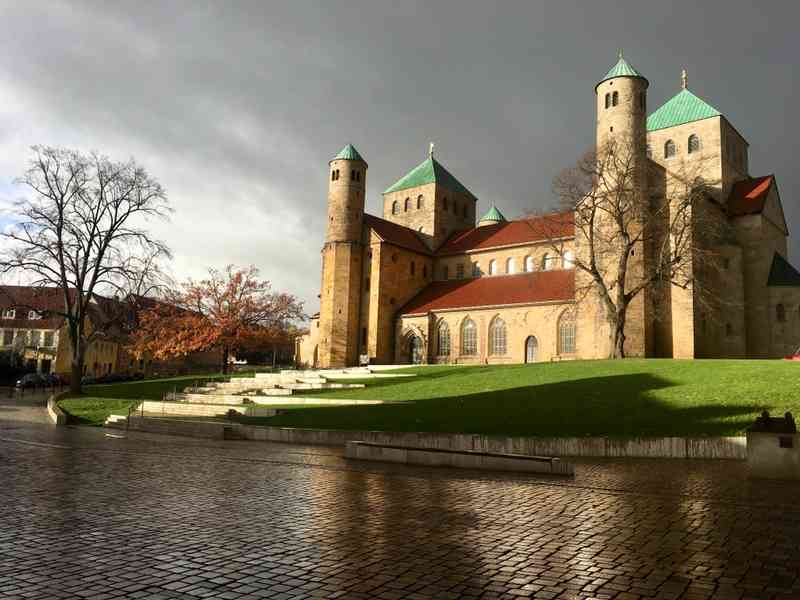
\includegraphics[width=1.0\linewidth]{05/hildesheim.jpg}
			}
		\end{minipage}
		\hfill
		\begin{minipage}{0.3\textwidth}
			
			\tcbox[colback=darkgray!85!black,
			left=0mm,right=0mm,top=0mm,bottom=0mm,boxsep=1mm,toptitle=0.5mm,bottomtitle=0.5mm,
			title=\centering{Maria Laach dóm}]{
				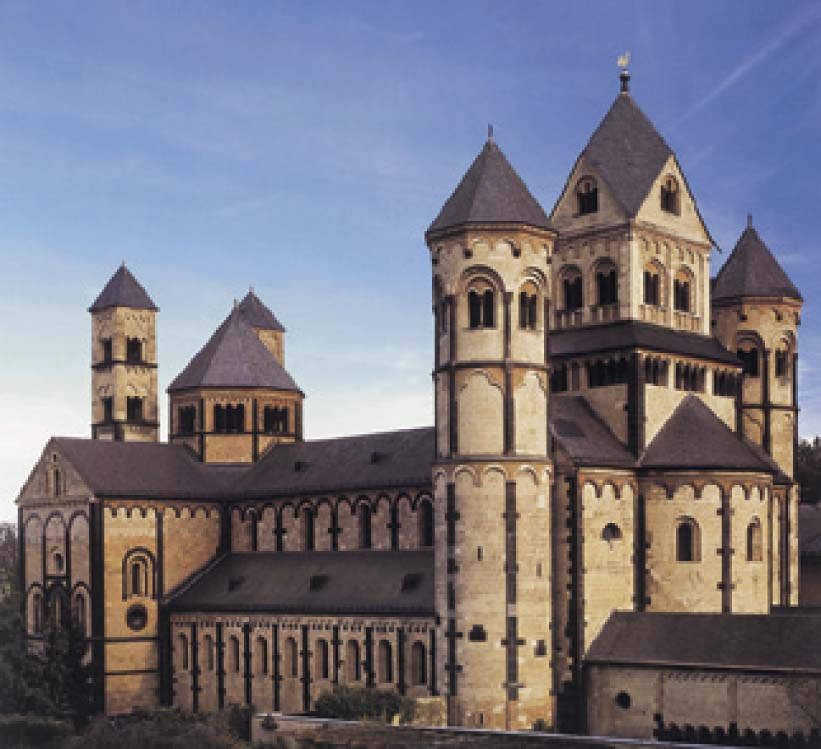
\includegraphics[width=1.0\linewidth]{05/maria_laach}
			}
		\end{minipage}
	\hfill
	\begin{minipage}{0.34\textwidth}
	
		\tcbox[colback=darkgray!85!black,
		left=0mm,right=0mm,top=0mm,bottom=0mm,boxsep=1mm,toptitle=0.5mm,bottomtitle=0.5mm,
		title=\centering{Speyer-i császárdóm}]{
			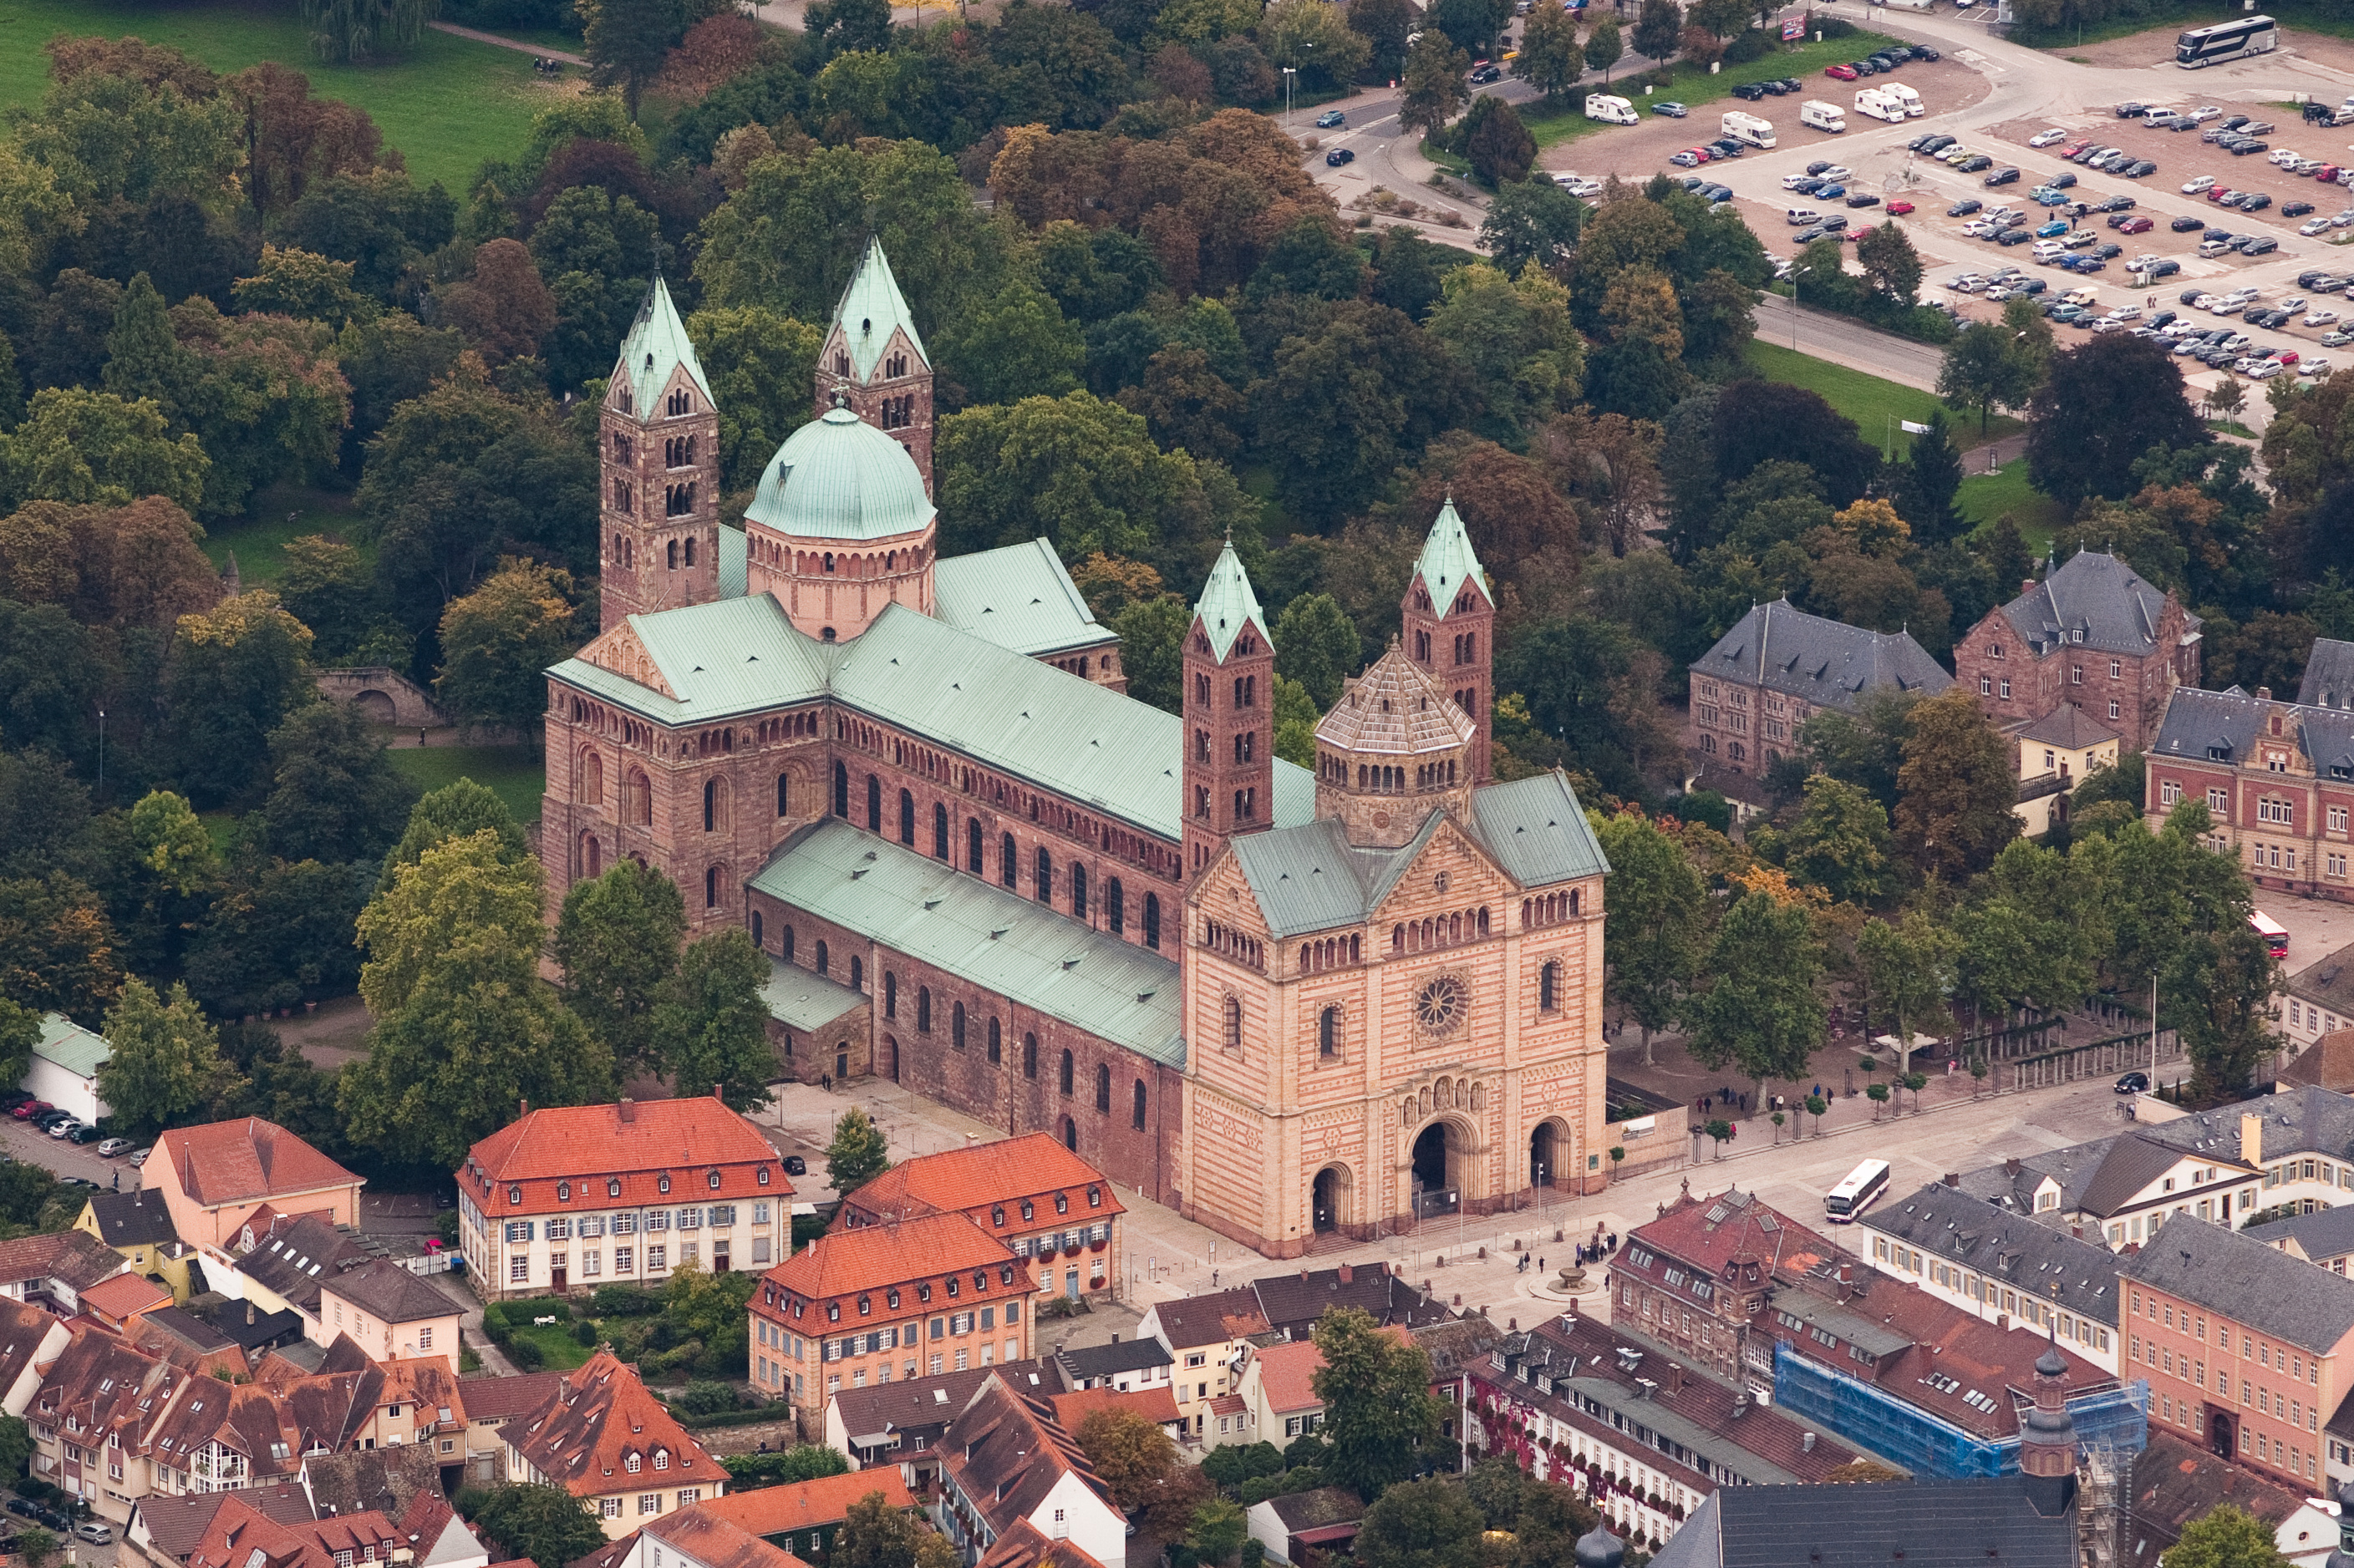
\includegraphics[width=1.0\linewidth]{05/speyer}
		}
	\end{minipage}
	\end{figure}
	
	
	\subsubsection{Itáliai építészet}
	
	\paragraph{Sajátosságai}
	Az itáliai építészet sajátosságai, hogy
	\begin{compactitem}
		\item a templomok három épületegységből állnak
		\item gyakori a márványburkolat
		\item gyakori az ún. „oroszlános kapuzat”
	\end{compactitem}

	\paragraph{Épületei}
	A templomhoz, azaz a dómhoz további két, külön álló épület kapcsolódik. A campanile, azaz harangtorony és a baptisztérium, azaz keresztelő kápolna. A kifejezés a latin baptistero (jelentése keresztelés) szóból ered. A
	baptisztérium olyan épület, ami a templom nyugati
	homlokzatával szemben áll, centrális alaprajzú, és benne
	egy szintén centrális keresztelő medence található a
	keresztelés szertartásának végzésére.
	
	A három részes román épületegyüttesek leghíresebb példája:
	a Pisa-i épületegyüttes.
	
	\paragraph{Pisai dóm}
	
	\subparagraph{Alaprajz}
	Alaprajza olyan mintha 3 bazilikából állna: 5-hajós hosszház + 2 háromhajós
	keresztház.
	
	\subparagraph{Külső tömeg}
	Hangsúlyos négyzeti tér alakul ki, ami fölött az itáliai
	építészetben a német templomok szögletes, sátortetős négyzeti tornyaitól
	eltérően íves, kupolához hasonló térlefedés van.
	
	\subparagraph{Homokzat}
	Legfőbb homlokzati díszek a törpegalériák (4 szinten), alul
	vakárkádok. A homlokzat teljes felületét márványburkolat díszíti
	
	\subparagraph{Belső tér} Márvány burkolat (csíkos), nyitott fa fedélszék
	
	\subparagraph{Szerkezet} Jól láthatóan bazilikás.
	
	\subparagraph{Pisai keresztelőkápolna (baptistérium)}
	Alaprajza kör alakú.
	
	Külseje követi a dóm díszítését - vakárkádos, törpegalériás ez is
	(a felső szintek már a gótika jegyében készültek, ezért felül fiatornyok, növényi faragványok is láthatók).
	
	
	
	\begin{wrapfigure}{r}{0.45\textwidth}
		\tcbox[colback=darkgray!85!black,
		left=0mm,right=0mm,top=0mm,bottom=0mm,boxsep=1mm,toptitle=0.5mm,bottomtitle=0.5mm,
		title=\centering{Pisa-i épületegyüttes}]{
			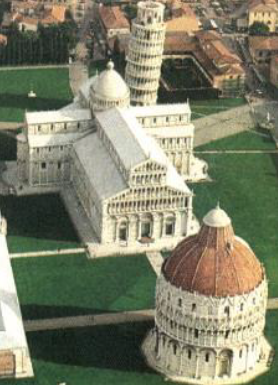
\includegraphics[width=1.0\linewidth]{05/pisa}
		}
	\end{wrapfigure}
	
	\subparagraph{Pisai "ferdetorony" (campanile)}
	Illeszkedik a dóm és a baptisztérium külső díszítéséhez: alul itt is vakárkádok, a felső szinteken törpegalériák találhatók; legfelül félköríves nyílások között a harangok; kör alaprajzú
		
	Már építése közben is elkezdett süllyedni, a 3 szint után megváltoztatták a dőlésszöget, hogy ne ferdüljön tovább, de már késő volt, az épület tovább süllyedt.
	
	\paragraph{Márványinkrusztáció}
	Az itáliai templomok különösen Firenzében elterjedt, gyakori díszítési módja a márványinkrusztáció, azaz színes márványlapokból kialakított burkolat. A márványlapok gyakran geometrikus mintát mutatnak, vagy faltagoló elemeket, pl. törpegalériát, ablakot, kapunyílást imitálnak.
	
	\paragraph{Oroszlános kapuzat}
	Észak-Itália templomainak leggyakoribb jellemzője az „oroszlános kapuzat”
	Az egyébként viszonylag díszítetlen templomhomlokzaton a kapu fölött baldachin található, aminek súlyát egy-egy oroszlánra támaszkodó oszlop tartja. A kaput őrző oroszlán motívuma a művészettörténetben a védelem szimbóluma.
	
	\subsubsection{A Cluny bencés apátság}
	
	\begin{wrapfigure}{r}{0.45\textwidth}
		\tcbox[colback=darkgray!85!black,
		left=0mm,right=0mm,top=0mm,bottom=0mm,boxsep=1mm,toptitle=0.5mm,bottomtitle=0.5mm,
		title=\centering{A Cluny bencés apátság makettje}]{
			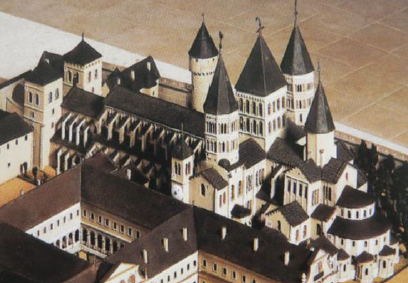
\includegraphics[width=1.0\linewidth]{05/cluny}
		}
	\end{wrapfigure}
	
	A román kori szerzetesi építészet jelentőségét, magas művészi értékét, gazdagságát a leghíresebb román kori szerzetesrend, a bencések \textbf{franciaország}i, Cluny-ben található kolostora példázza. A hatalmas épületegyüttesből mára mindössze a nagyobbik kereszthajó déli szárnya maradt meg, a többi rész robbantások áldozata lett. Az egykori impozáns épületegyüttesről rekonstrukciós rajzok és makettek alapján tájékozódhatunk.
	
	A bencés apátságok önálló, saját gazdasággal rendelkező kisvárosok voltak. Természetesen központjukban mindig a templom állt, amellett volt található a kolostor épülete.
	
	\paragraph{Kolostor-templom}
	Hatalmas méretű, monumentális épület volt: hosszháza 5 hajóból állt, amihez 3 hajós (!) előcsarnok csatlakozott, továbbá a templomnak 2 keresztháza volt. Az alaprajz tehát bonyolult volt, nagyon gazdag, számos kis épületrészből állt.
	
	\paragraph{A kolostor részei}
	A templomokhoz kapcsolódó kolostorok mindig azonos rend, alaprajz szerint épültek fel.
		
		\subparagraph{Kerengő}
		Azz ókeresztény átrium teréből kialakuló, elmélkedésre szolgáló, négyzet alaprajzú, árkádos folyóval körbevett udvar volt a központ.
		
		\subparagraph{Reflektórium}
		A kerenmgőből nyíló szerzetesi ebédlő, ált. egy hosszúkás terem.
		
		\subparagraph{Dormitórium}
		Szintén a kerengőből nyíló, szerzetesi alvóhely.
		
	A kolostorhoz konyha, temető, kórház, gazdasági egységek, vendégház, istálló, kert, veteményes, pékség, és további, az önálló szerzetesi élethez szükséges épületek csatlakoztak.
	
	\subsection*{Szobrászat}
	
		A szobrászati alkotások az épületekhez kapcsolódnak, domborművek (csak ritka esetben szabadon álló körplasztikák).
		\begin{compactitem}
			\item Az épület nyugati homlokzatán található domborművek.
			\item A kapu fölötti íves timpanonban lévő domborművek.
			\item Figurális oszlopfejezetek az épületbelsőben.
		\end{compactitem}
	
		\paragraph{Stílus}
		\begin{compactitem}
			\item anyaga kő
			\item a téma mindig vallásos
			\item a kompozíció egyszerű, zsúfolt
			\item nincsen valós térbeliség, térmélység, síkszerű az ábrázolás
			\item a figurák nem reálisak, nem életszerűek (,,primitívek”)
			\item a drapériaredőzés stilizált, vonalas
			\item a testtartások életszerűtlenek
			\item a mozdulatok, a gesztusok viszont kifejezőek, mindössze ezek teszik érthetővé a történeteket
			\item a tekintetek semmitmondóak
			\item a kompozíció az épülethez kapcsolódik, nincsenek szabadon álló szobrok, a fő műfaj a dombormű
			\item ragaszkodik a bibliai szöveghez, többletet nem fűz hozzá (nem célja, hogy hasson a néző érzelmeire, sem, hogy értelmezze a szöveget, sem, hogy saját gondolatot fűzzön hozzá), hanem az írástudatlan hívő számára megjeleníti, elmeséli a bibliai történeteket, ,, Biblia pauperum”, azaz a ,, Szegények Bibliája” volt a szobrász.
		\end{compactitem}
		
		\paragraph{Domborművek a homlokzatokon}
		Térmélységet nem jelentő falsík előtt jelennek meg a tömbszerűen összefogott figurák. Az előadásmód epikus, elbeszélő jellegű. A mozdulatok, testtartások egyszerűek, de ezek a kifejező gesztusok mesélik el a történetet.
		
		A figurák álltalában egyformák, felismerhetetlenek.
		
		\begin{wrapfigure}{r}{0.45\textwidth}
			\tcbox[colback=darkgray!85!black,
			left=0mm,right=0mm,top=0mm,bottom=0mm,boxsep=1mm,toptitle=0.5mm,bottomtitle=0.5mm,
			title=\centering{Maestes domini dombormű}]{
				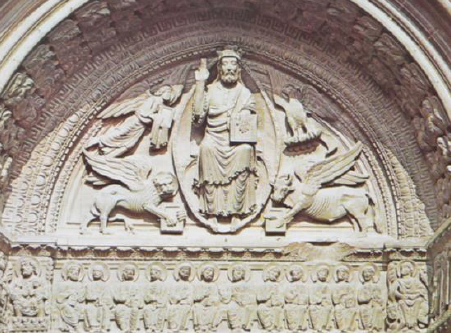
\includegraphics[width=1.0\linewidth]{05/maestes_domini}
			}
		\end{wrapfigure}
		
		\paragraph{Domborművek a kapuk fölötti ívháromszögben}
		Leggyakoribb témája az ún. Maestas Domini, azaz ,,Fenséges Úr” = János apostolnak a Jelenések könyvében vagy más néven az Apokalipszis-ben található víziója. Leghíresebb példa:
		Arles, Saint Trophim (árli szen trofim) ívtimpanonja Franciaország.
		
		A téma kialakulásának oka az lehetett, hogy 1000 körül - mivel kerek évszám - igen erős volt a végidő-várás, így nem csoda, hogy egy azzal összefüggő, arra utaló látomás készült leggyakrabban a templomok bejárata fölé.
		
		\paragraph{Figurális oszlopfejezetek}
		Az érett román korban eltűnnek a kockafejezetek, helyettük az épületbelsőben gyakran plasztikusan kifaragott figurális kompozíciók jelennek meg az oszlopok tetején. Ezek általában szörnyeket, ijesztő állatfigurákat, a büntetésre utaló bibliai történetek bukott, pokolra jutott alakjait mutatják.
		
	\clearpage
	
	\subsection*{Magyar román kor}
	
	\begin{figure}[H]
		\centering
		\begin{minipage}{0.47\textwidth}
			\tcbox[colback=darkgray!85!black,
			left=0mm,right=0mm,top=0mm,bottom=0mm,boxsep=1mm,toptitle=0.5mm,bottomtitle=0.5mm,
			title=\centering{Jáki templom}]{
				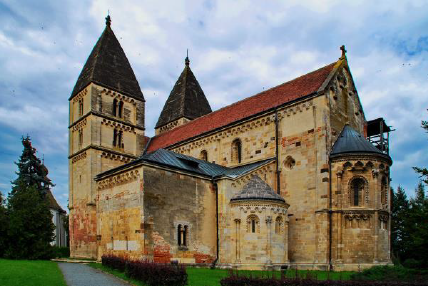
\includegraphics[width=1.0\linewidth]{05/jak}
			}
		\end{minipage}
		\hfill
		\begin{minipage}{0.47\textwidth}
			
			\tcbox[colback=darkgray!85!black,
			left=0mm,right=0mm,top=0mm,bottom=0mm,boxsep=1mm,toptitle=0.5mm,bottomtitle=0.5mm,
			title=\centering{Pécsi székesegyház}]{
				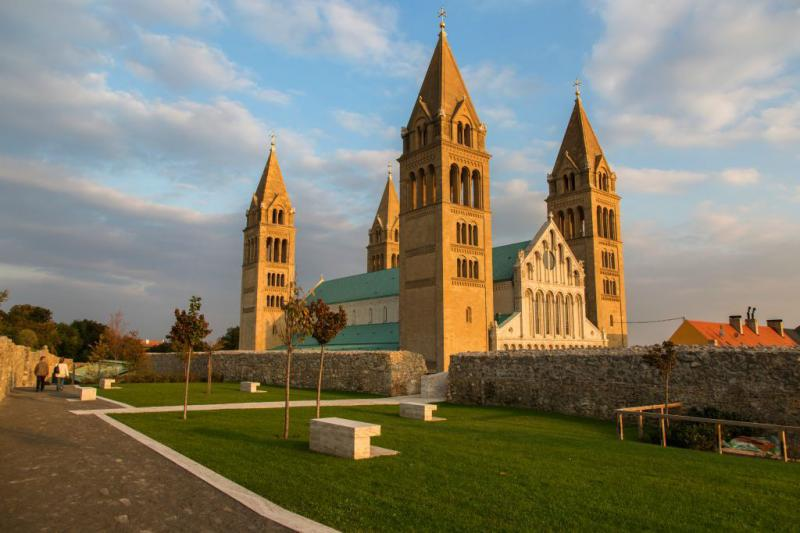
\includegraphics[width=1.0\linewidth]{05/pecs_szekesegyhaz}
			}
		\end{minipage}
	

		\begin{minipage}{0.7\textwidth}
			
			\tcbox[colback=darkgray!85!black,
			left=0mm,right=0mm,top=0mm,bottom=0mm,boxsep=1mm,toptitle=0.5mm,bottomtitle=0.5mm,
			title=\centering{Szent István szarkofág}]{
				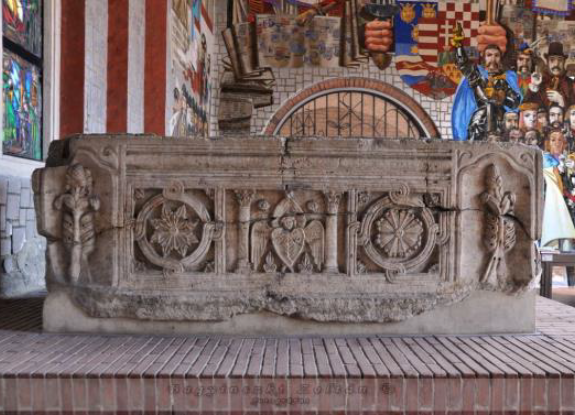
\includegraphics[width=1.0\linewidth]{05/szent_istvan_szarkofag}
			}
		\end{minipage}
	\end{figure}
	
	

\cleardoublepage


\section{A románkori freskófestészet, kódexfestészet és alapozási technikák}

\begin{center}
	\begin{longtable}{ | p{0.25\textwidth} | p{0.75\textwidth} | }
		
		\hline
		\multicolumn{2}{|c|}{\textbf{A tétel adatai}}
		\\ \hline
		
		\hline
		\centering{Tétel teljes címe}
		&
		Milyen hasonlóságokat és különbségeket talál a román kori freskófestészet és a kódexfestészet között tartalmilag, formailag és technikailag? Mutassa be a középkorban elterjedt alapozási technikákat, pigmenteket, kötőanyagokat!
		\\ \hline
		
	\end{longtable}
\end{center}

\subsection*{Románkori festészet}

A román kori festészet kezdetét az építészetével és a szobrászatával együtt az ezredfordulóra teszik. A falfestészetből nagyon kevés és rossz állapotú emlékanyag maradt az utókorra. 

\subsection*{Kódexfestészet}

\begin{wrapfigure}{r}{0.4\textwidth}
	\tcbox[colback=darkgray!85!black,
	left=0mm,right=0mm,top=0mm,bottom=0mm,boxsep=1mm,toptitle=0.5mm,bottomtitle=0.5mm,
	title=\centering{Oroszlán Henrik evangeliáruma, 12. század}]{
		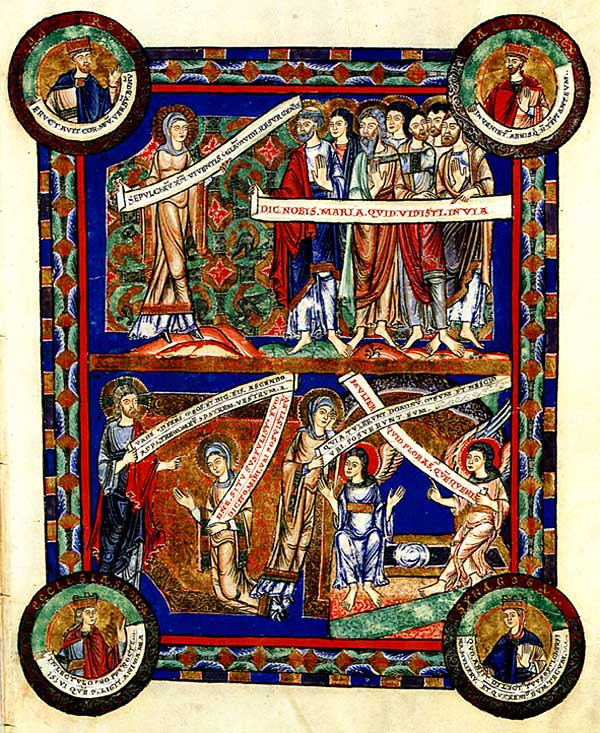
\includegraphics[width=1.0\linewidth]{05/kodex}
	}
\end{wrapfigure}

Jelentősen megnövekedett a művészetpártoló világiak száma, az uralkodó mellett már a nemesek is rendeltek értékes kódexeket.

A középkori könyvfestészet leggyakoribb témája Krisztus élete, csodái és szenvedéstörténete. Legtöbbször az evangeliárumokat díszítették ezekkel, melyek teljes egészében vagy részleteikben tartalmazták az evangéliumokat. Krisztus szenvedéseit általában kevésbé hangsúlyozták, pl. az Ottó-korban hagyományosan Krisztus csodáira helyezték a hangsúlyt. A kódexekben sosem törekedtek Krisztus teljes életének illusztrálására, és a megbízók a Megváltó életének pozitív eseményeit akarták látni, hatásos, reprezentatív formában. Esztétikailag "eladhatóvá" akarták tenni az üdvtörténetet. Ez arra utal, hogy az egyház nagy súlyt fektetett a -mai szóval élve- propagandára.

\subsection*{Románkori freskófestészet}

	\begin{wrapfigure}{r}{0.5\textwidth}
	\tcbox[colback=darkgray!85!black,
	left=0mm,right=0mm,top=0mm,bottom=0mm,boxsep=1mm,toptitle=0.5mm,bottomtitle=0.5mm,
	title=\centering{Románkori Maestes domini témájú freskó}]{
		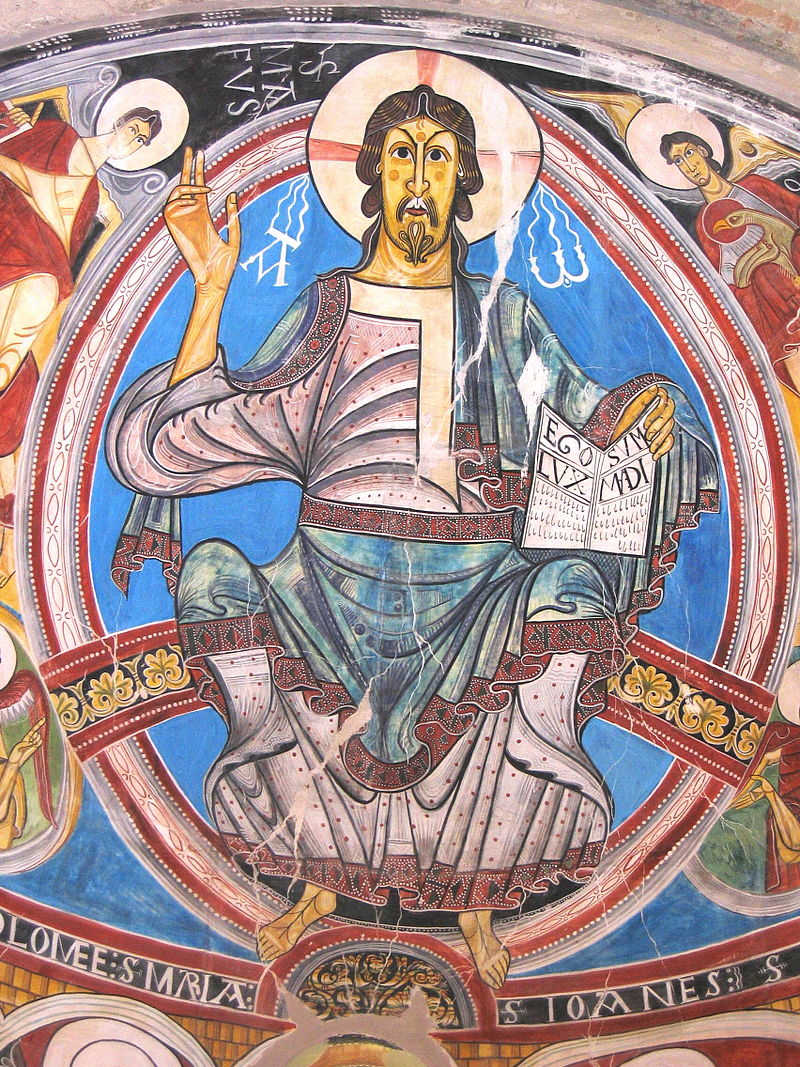
\includegraphics[width=1.0\linewidth]{05/fresko}
	}
\end{wrapfigure}

A korai román-kori festészetben gyakran alkalmazták a könyvfestészet kompozíciós megoldásait és motívumait. A kéziratok gyorsan terjedtek, a mérvadó központokban legkésőbb a 11. században már ismerték a fontosabb kódexeket. Az érett középkorban már nemzetközi stílusról beszélhetünk, a művészek vándoroltak, különböző uralkodók és főpapok megrendelésére dolgoztak.

A román-kori festészet egy sajátos formája a cakkos stílus, egy különös és rövid életű stílusirányzat. Jellemző rá, hogy a figurák ruhájának szegélye szokatlanul éles szögben törik meg, a formák szinte manierista stilizálása átmenetet teremt a gótika festészetéhez.

\subsection*{A freskó- és kódexfestészet összehasonlítása}

\paragraph{Különbségek}
A kódexfestészetben a könyvekbe kerülő miniatúrák kisebb méretüknél fogva drágább pigmentek felhasználásával is készülhetett, így azok színei élénkebbek.

A kódexekre jellemzőek voltak az iniciálék, a díszes betűk használata.

A méretüknél fogva részletgazdagságukban is különböztek.

\paragraph{Hasonlóságok}

Mind a kódexfestészetnek, mind a freskófestészeneklt a korra jellemző apátságok, szerzetesrendek kolostorai voltak a központjai.

Mind a kettőre jellemző volt a dekoratív színhatás, síkszerű ábrázolásmód, a narratív, elbeszélő előadásmód (ugyan ez jellemző volt a domborművekre is).

Mindkettő esetében meghatározó eszmei háttér a kereszténység, témáik bibliai történetek, szentek, vértanúk élete volt.

Mindkettőre jellemzőek voltak a díszítő motívumok, és sötét kontúrok.

\paragraph{Alapanyagok}

	A kódexfestészethez tojástemperát használtak, ásványi festékeket és növényi olajokat.
	
	A freskó esetében mészálló festékre volt szükség: fémoxidok, földfestékek.

\subsection*{A freskó}

	\subsubsection{Alapanyagok}
	
	Gipsz, mészhabarcs alapozás.
	
	Csak mészálló festékek használhatók, elsősorban fémoxidok, földfestékek, ez behatárolja a rendelkezésre álló színskálát.
	
	\subsubsection{Menete}
	
	\begin{itemize}
		\item A freskófestészet meghatározó törvénye, hogy a vakolat és a mészfesték viszonylag hamar megköt, tehát 6–8 óra alatt a munkát be kell fejezni, utólagos finomításokra már nincs mód.
		
		\item Nagyobb felületű képek készítése tehát csak kisebb, egy nap alatt elkészíthető adagokban (giornate) lehetséges, egyszerre mindig csak néhány négyzetméternyi felületet készítenek elő, majd festenek meg.
		
		\item A karton vázlat: Az előbbiekből következik, hogy a munka megkezdésekor már tökéletesen kiforrott elképzeléssel, tervekkel kell rendelkeznie a művésznek, és ezt minél gyorsabban meg kell tudnia valósítani. Ennek érdekében legtöbbször eredeti (1:1-es méretű) nagyságú vázlatot, kartont készítenek, amelyet majd a helyszínen a festés megkezdése előtt „pauzálnak”, a felületre átmásolnak. Ennek különösen nagy jelentősége van akkor, ha a befestendő felület geometriailag bonyolult formájú, például egy kupola belső felülete.
	\end{itemize}

	\paragraph{Lépései}
	
	\begin{enumerate}
		\item Alapozás: A freskó hordozója a vakolat, ennek minősége határozza meg az egész mű tartósságát.
		\begin{compactitem}
			\item Először le kell verni tégláig a régi, alkalmatlan vakolatot a falról. Majd kikaparjuk a fugákat. Az alapozás a csupasz téglafal benedvesítésével kezdődik.
			
			\item Maj erre kerül több rétegben a friss vakolat.
		\end{compactitem}
	
		\item Festés: A festés a harmadik réteg vakolatra kerül, annak felhordása után kb. egy óra múlva kell megkezdeni, és 6-8 óra alatt be is kell fejezni. 
		
		\item Ezután a nedves falból, illetve a vakolatból kifelé szivárgó meszes víz a kép felszínén szétterül, és a levegővel érintkezve vékony mészpáncélt alkot.
		
		\item A javítás ezután csak a vakolat teljes leverése és újraalapozása után lehetséges. Teljes száradás után a színek áttetsző mészkőkristályokba dermedve szinte örök életűek.
	\end{enumerate}

\paragraph{Története}

	A legkorábbi ismert al fresco készült falfestmények kb. i. e. 1500-ból származnak, Kréta szigetén a knósszoszi palotában találhatók, de Pompejiből is maradtak fenn kitűnő állapotban lévő freskók. Fénykora az itáliai reneszánszban volt. A freskó technikája az évezredek során szinte semmit se változott, mivel bebizonyította rendkívüli tartósságát.

